\chapter{Проникновение решетки вихрей в объем} \label{chapt6}

В предыдущих главах было описано исследование вихревого движения волнами на поверхности жидкости, а так же представлена теоретическая модель, описывающая данное явление. Как известно \cite{land} волновое движение проникает в глубину жидкости, убывая с экспоненциальные законом 
\begin{equation}
 \label{eq:deepWave}
H(z) = H(0) e^{-kz},
\end{equation}
 где $z$ - глубина, а $k$ - волновой вектор. Однако согласно построенной модели вихревое движение будет генерироваться в объеме по несколько другому закону. Сначала вспомним, что согласно построенной модели есть два механизме генерации вихревого движения. 
	Первый, более простой, заключается в переносе пробных частичек в результате дрейфа Стокса. Согласно ему вихревое движение возникает сразу в каждой точке, где появляется волны, и исчезает сразу же как волны затухают или уходят из исследуемой области. Т.е. согласно формулам (\ref{eq:deepWave}) и (\ref{eq:vortStand}) проникновение вихрей возникающих из-за дрейфа Стокса в глубину должно быть так же экспоненциальным, однако с вдвое большим показателем экспоненты.
\begin{equation}
 \label{eq:deepStocks}
\Omega_{St}(z)  = e^{-2kz} sin \phi H_x(0) H_y(0) \omega k^2 sin(kx)sin(ky)
\end{equation}
Стоит также отметить, что из-за того, что дрейф Стокса наблюдается в лагранжевых координатах, но не в эйлеровых \ref{p1_lagr}, то это вихревое движение не имеет инерции и не существует отдельно от волн.
	Второй механизм отвечающий за генераций вихрей волновым движение описывает генерацию именно завихренности в эйлеровых координатах. Согласно ему завихренность возникает в результате нелинейного взаимодействия волн в тонком вязком приповерхностной подслое. Для волн частотой 3 Гц на поверхности воды его толщина будет около \todo{вставить формулу и ссылку на литературу} 200 мкм. Что безусловно мало по сравнению с длиной и даже амплитудой волны, однако больше, чем характерный размер 30 мкм декорирующией частички полиамида-12. В объем же завихренность из-за этого механизма попадет диффузный образом, за счет вязкого трения между слоями жидкости. Таким образом в стационарном режиме предсказывается тоже экспоненциальное распределение завихренности по глубине:
\begin{equation}
 \label{eq:deepEyler}
\Omega_N(z)  = \sqrt{2}e^{-\sqrt{2}kz} sin \phi H_x(0) H_y(0) \omega k^2 sin(kx)sin(ky)
\end{equation}

Приведенные теоретические оценки (\ref{eq:deepStocks}, \ref{eq:deepEyler}) показывают, что несмотря на то, что размер вихрей составляет пол длины волны $\sim 8$ см, падение амплитуды решетки в е раз стоит ожидать уже на глубине $h = 1/2k \sim 1.4$ см. Исходя из этой оценки был выбран набор глубин, на которых производится наблюдение за динамикой решетки вихрей: от 0.5 см до 3.5 см.

Так же можно оценить скорость диффузии завихренности в глубину из вязкого подслоя. \todo{оценка}

\section{Экспериментальная методика} \label{sect6_2}
Для регистрации завихренности в объеме жидкости используется методика лазерного листа. Для декорации вихревого движения в объем вводятся частички полиамида-12, чья плотность близка к плотности воды. Частички подсвечивается лазерным листом, который получается пропусканием луча от лазера MGL H 532-500mW мощностью 0,5 Вт  через цилиндрическую линзу диаметром 0.6 см, установленную вертикально. После прохождения линзу лучом, он раскрывался в горизонтальный лазерный лист толщиной около 1 мм. Лазерный лист подсвечивает только те частицы в объеме, которые встречаются на его пути. Таким образом можно декорировать течения в объеме жидкости лежащие в плоскости лазерного листа. Видеосъемка частиц производилась также камерой Canon 70D. Пример получившегося кадра показан на рис \ref{img:track0p5cm}. Пример поля завихренности показан на рисунке \ref{img:vort0p5cm}.
\begin{figure}[ht]
  \center{\includegraphics[width=.9\linewidth]{part6/track0p5cm.jpg}}
  \caption{Кадр видеосъемки 40х70 см$^2$ частиц полиамида, подсвеченных лазерным листом в горизонтальном слое на глубине 0.5 см.}
  \label{img:track0p5cm}  
\end{figure}

\begin{figure}[ht]
  \center{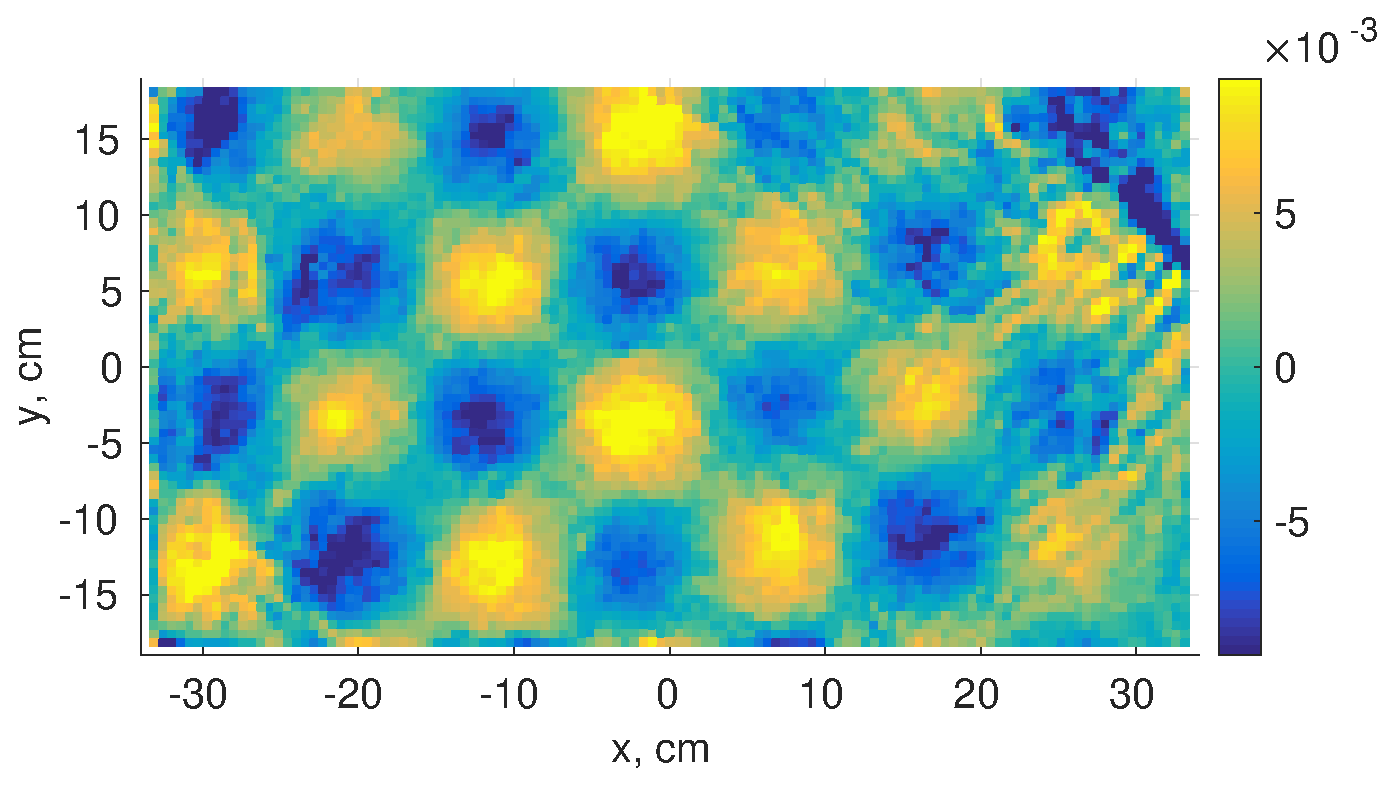
\includegraphics[width=.9\linewidth]{part6/vort0p5cm.eps}}
  \caption{Фрагмент 40х70 см$^2$ поля вертикальной завихренности в горизонтальном слое на глубине 0.5 см.}
  \label{img:vort0p5cm}  
\end{figure}


\section{Экспериментальные результаты} \label{sect6_3}

В первом эксперименте было произведено 5 измерений на разных глубинах: 0.5 см, 1.25 см, 2.0 см, 2.75 см, 3.5 см. Накачка производилась на частоте 3 Гц. На каждой глубине измерялась амплитуда завихренности решетки вихрей в течении 600 секунд после включении накачки. На рисунке 4 показаны зависимости амплитуд завихренности решетки вихрей от времени для каждой глубины(более маленькой глубине соответствует более высокая кривая на рисунке). Так же черной кривой показана зависимость $1.4 \cdot 10^{-2} - 8 \cdot 10^{-3} e{-t/165}$. Т.е. на глубине 0.5 см завихренность росла с характерным временем 165 с. Оценка характерного времени роста завихренности для других глубин так же дают характерные времена около 200 с. Колебания амплитуды завихренности, которые видны до 200 секунды, связаны с переходными процессами установления волн на поверхности воды. Так как накачка производится на частоте немного отличающейся от резонансной частоты системы, то в процессе установления стоячей волн происходят биения с характерной частотой равной разности частот вынуждающей силы и собственных колебаний системы.

\begin{figure}[ht]
  \center{\includegraphics[width=1\linewidth]{part6/5deeps.jpg}}
  \caption{Зависимость завихренности решетки вихрей от времени, на глубинах 0.5 см, 1.25 см, 2.0 см, 2.75 см, 3.5 см. Черная кривая соответствует зависимости $1.4 \cdot 10^{-2} - 8 \cdot 10^{-3} e{-t/165}$.}
  \label{img:5deeps}  
\end{figure}

Полученные графики стоит сравнить с динамикой возникновения завихренности на поверхности воды. 
\todo{динамика на поверхности воды!}

Для понимания проникновения структуры вихрей в глубину рассмотрим Фурье образ поля завихренности на разных глубинах в начальный интервал времени (50-100 секунд после включения накачки) и через 10 минут после включения накачки (550-600 секунды). Соответствующие графики показаны на рисунках \ref{img:detphFFT} а-е. На рисунках видно, что в один и тот же интервал времени структура завихренности на разных глубинах одинаковая, однако она меняется со временем. Это изменение можно связать с тем, что помимо решетки вихрей в жидкости возбуждаются крупномасштабные вихри, которые сносят  решетку завихренности продиффундировавшей из вязкого подслоя.

\begin{figure}[ht]
  \begin{minipage}[ht]{0.326\linewidth}
    \center{\includegraphics[width=1\linewidth]{part6/UnderFFT/Under_scan3Hz25mV600s0p50cm_050s.eps} \\ а) t = 50 с, h = 0.5 см}
  \end{minipage}
  \hfill
  \begin{minipage}[ht]{0.326\linewidth}
    \center{\includegraphics[width=1\linewidth]{part6/UnderFFT/Under_scan3Hz25mV600s2p00cm_050s.eps} \\ б)  t = 50 с, h = 2.0 см}
  \end{minipage}
  \begin{minipage}[ht]{0.326\linewidth}
    \center{\includegraphics[width=1\linewidth]{part6/UnderFFT/Under_scan3Hz25mV600s3p50cm_050s.eps} \\ в)  t = 50 с, h = 3.5 см}
  \end{minipage}
  \begin{minipage}[ht]{0.326\linewidth}
    \center{\includegraphics[width=1\linewidth]{part6/UnderFFT/Under_scan3Hz25mV600s0p50cm_550s.eps} \\ г) t = 550 с, h = 0.5 см}
  \end{minipage}
  \hfill
  \begin{minipage}[ht]{0.326\linewidth}
    \center{\includegraphics[width=1\linewidth]{part6/UnderFFT/Under_scan3Hz25mV600s2p00cm_550s.eps} \\ д) t = 550 с, h = 2.0 см}
  \end{minipage}
  \begin{minipage}[ht]{0.326\linewidth}
    \center{\includegraphics[width=1\linewidth]{part6/UnderFFT/Under_scan3Hz25mV600s3p50cm_550s.eps} \\ е) t = 550 с, h = 3.5 см}
  \end{minipage}  
  \caption{Фурье образ поля завихренности на разных глубинах а-в) в начальный момент времени (50-100 секунд после включения накачки) и г-е) через 10 минут после включения накачки (550-600 секунды).}
  \label{img:detphFFT}  
\end{figure}



На рисунке \ref{img:depth} показан график зависимости завихренности в промежуток времени от 500 до 600 секунд после включения накачки от глубины. Черная прямая соответствует зависимости $e^{-2kh}+\sqrt{2}e^{-\sqrt{2}kh}$, где k = 0.36 см$^{-1}$, зеленая прямая - $2 \cdot 10^{-2} e^{-2kh}$. Как видно по рисунку разброс экспериментальных точек не позволяют однозначно соотнести их с одной или другой экспоненциальной зависимостью. Так же стоит отметить, что снос завихренности решетки вихрей из-за развития крупномасштабных течений так же уменьшает вклад решетки завихренности продиффундировавшей из вязкого подслоя. Что в свою очередь тоже может объяснять отличие экспериментальных точек от зависимости \ref{eq:deepEyler}.

\begin{figure}[ht]
  \center{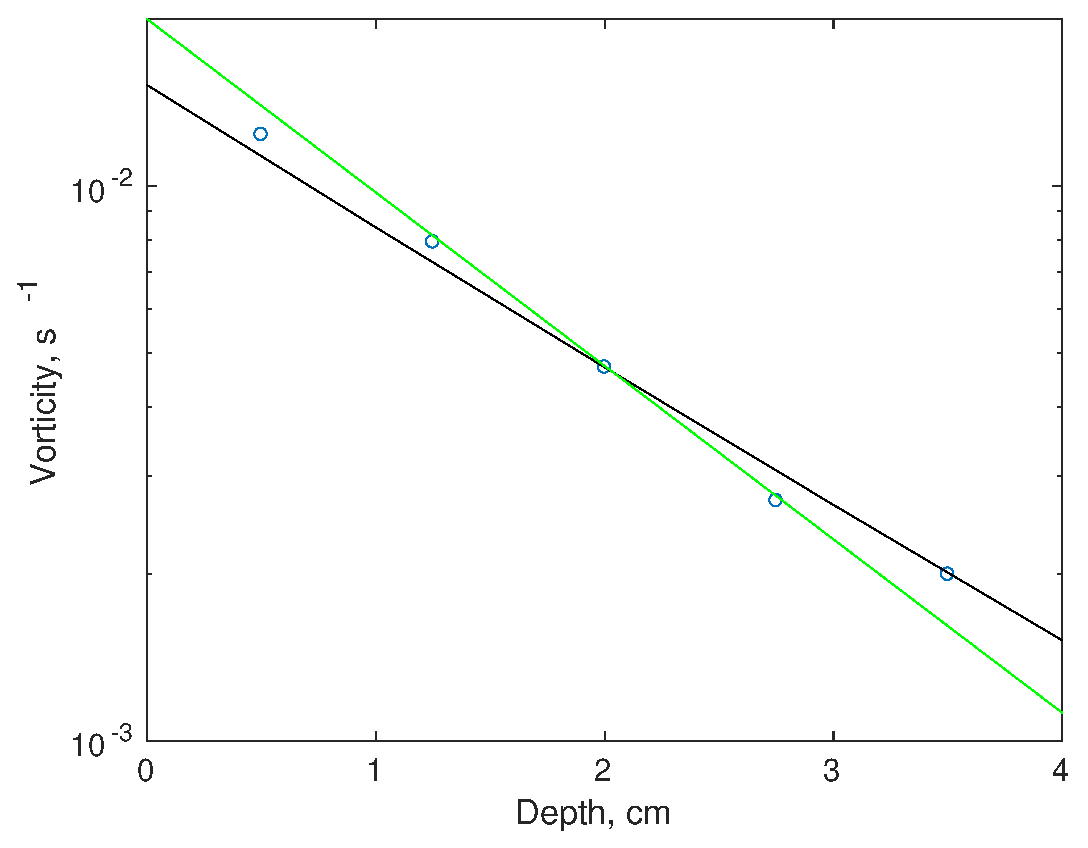
\includegraphics[width=.5\linewidth]{part6/depth.eps}}
  \caption{Зависимость завихренности решетки вихрей от глубины. Черная прямая соответствует зависимости $6.3 \cdot 10^{-3} (e^{-2kh}+\sqrt{2}e^{-\sqrt{2}kh})$, зеленая прямая - $2 \cdot 10^{-2} e^{-2kh}$}
  \label{img:depth}  
\end{figure}

\section{Обсуждение экспериментальных результатов} \label{sect6_4}
\section{Выводы} \label{sect6_5}
Экспериментально показано, что в объеме решетка вихрей структуру и зависимости амплитуды от в глубины близка к  экспоненциальному закону $e^{-2kh}$, где k — волновой вектор возбуждаемой решетки, а h — глубина слоя жидкости. 

Экспериментально оценено характерное время 200 секунд проникновения завихренности решетки вихрей из вязкого подслоя в объем.

Экспериментально показано, что наличие крупномасштабных вихрей приводит к «сносу» завихренности, проникающей в объем из вязкого подслоя. При этом величина завихренности решетки вихрей  близка к вкладу завихренности возникающего из-за дрейфа Стокса.
\clearpage